\documentclass[10pt]{article}

\usepackage[utf8]{inputenc}
\usepackage[american]{babel}
\usepackage{graphicx}
\usepackage{amsmath}
\usepackage{amsthm}
\usepackage{amssymb}
\usepackage{natbib}
\usepackage[margin=0.5in]{geometry}
\usepackage{fancyvrb}
\usepackage{Sweave}

\DefineVerbatimEnvironment{Sinput}{Verbatim}{xleftmargin=2em}
\DefineVerbatimEnvironment{Soutput}{Verbatim}{xleftmargin=2em}
\DefineVerbatimEnvironment{Scode}{Verbatim}{xleftmargin=2em}
\fvset{listparameters={\setlength{\topsep}{0pt}}}
\renewenvironment{Schunk}{\vspace{\topsep}}{\vspace{\topsep}}

\setlength{\parskip}{.1in}  
\setlength{\parindent}{0.0in}  

\setcounter{tocdepth}{1}
%\setcounter{secnumdepth}{1}

\newcommand{\R}{\textsf{R}}
\newcommand{\code}[1]{\texttt{#1}}
  
%\SweaveOpts{eps=FALSE, pdf=TRUE, png=TRUE, keep.source=FALSE, echo=TRUE, eval=TRUE}
  
\title{Ecological geometry of Africa}
\author{John M. Drake}
  
\begin{document}
\Sconcordance{concordance:niche-space.tex:niche-space.Rnw:%
1 47 1 1 2 4 0 1 2 2 1 1 2 1 0 4 1 1 2 5 0 1 2 2 1 1 2 1 0 1 1 1 2 1 0 %
1 2 1 0 1 2 5 0 1 2 4 1}


\maketitle
  
\section{Introduction}
  
My studies of mosquito distributions in Africa have routinely yielded two interesting phenomena: (1) at least two species (\textit{Anopheles arabiensis} and \textit{Culex pipiens}) are climate generalists in the space of the first two principal components of environmental space, and (2) the set of environmental conditions appears as a ``ring'' in the first two principal components and a ``sheet'' in three principal components.

The purpose of this study is to seek to understand this phenomena better.

\section{Exploratory plots}

First we load data from the ongoing study of \textit{Cx. pipiens}. 

\begin{Schunk}
\begin{Sinput}
> load('culex-v4.RData')
\end{Sinput}
\end{Schunk}

Now we plot the familar pca plot of environmental conditions in Africa where the scatterplot is resutricted to 2000 observations to better show the ``ring''. To ensure that these are not ordered in any way, these points are chosen randomly.

\begin{Schunk}
\begin{Sinput}
> par(mfrow=c(2,1))
> plot(pca, main='Scree plot', cex.main=0.5)
> set.seed(10281979)
> n <- dim(pca$x)[1]
> pca.sample <- pca$x[sample(seq(1,50000),5000),]
> plot(pca.sample[,1:2], main='Principal Components Analysis (n=2,000)',
+      pch=19, cex=0.02, col='grey', cex.main=0.5, xlab='PC1', ylab='PC2')
\end{Sinput}
\end{Schunk}
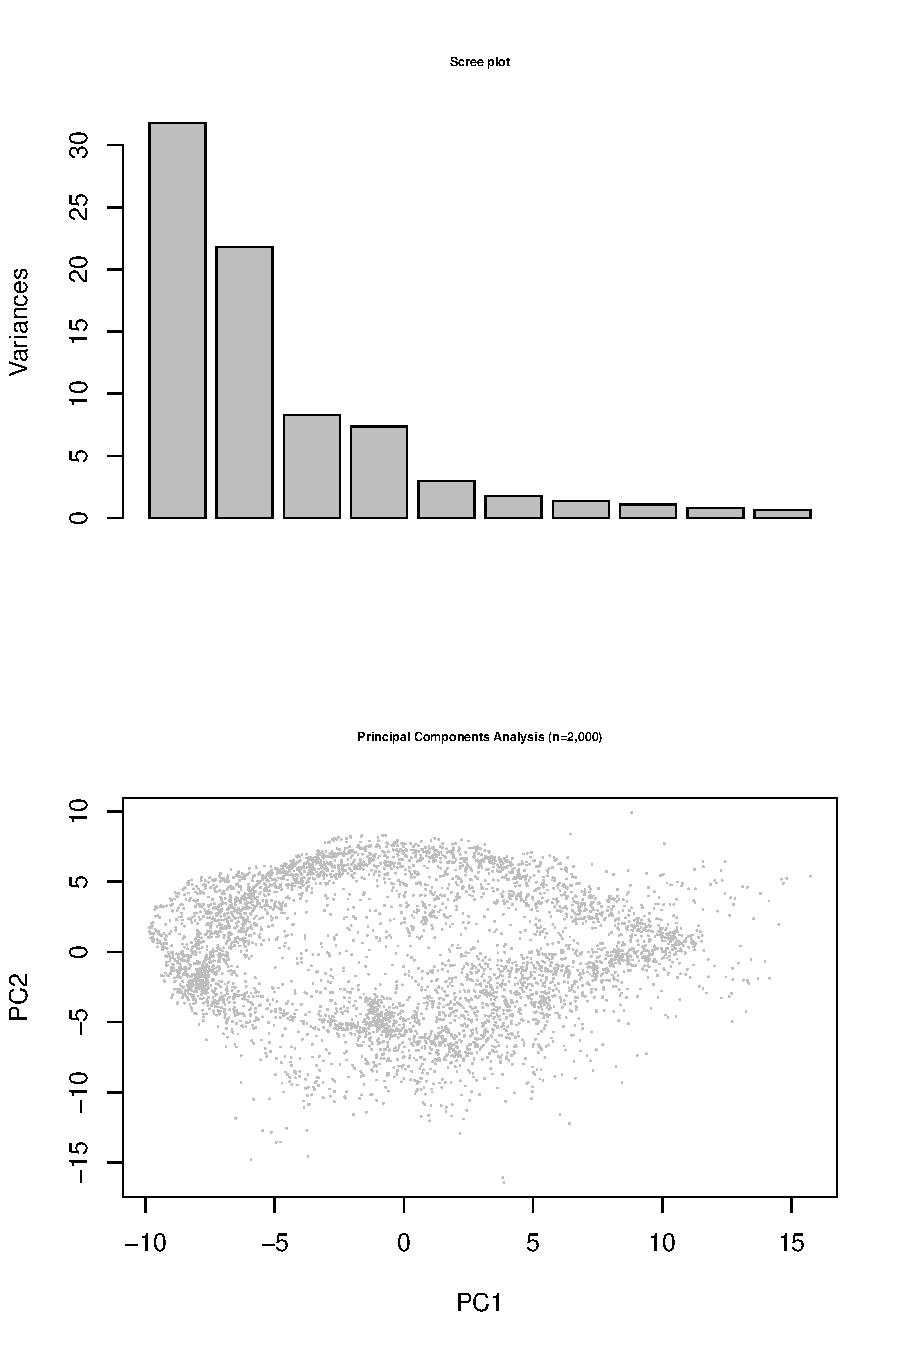
\includegraphics{niche-space-screeplot}

Now, we again inspect the plot in three dimensions

\begin{Schunk}
\begin{Sinput}
> require(scatterplot3d)
> par(mfrow=c(3,1))
> scatterplot <- scatterplot3d(pca.sample[,1:3], pch=19, cex.symbols=0.2, type='p',
+                              highlight.3d=TRUE, xlab='PC1', ylab='PC2', zlab='PC3', angle=45)
> scatterplot <- scatterplot3d(pca.sample[,1:3], pch=19, cex.symbols=0.2, type='p',
+                              highlight.3d=TRUE, xlab='PC1', ylab='PC2', zlab='PC3', angle=100)
> scatterplot <- scatterplot3d(pca.sample[,1:3], pch=19, cex.symbols=0.2, type='p',
+                              highlight.3d=TRUE, xlab='PC1', ylab='PC2', zlab='PC3', angle=-20)
\end{Sinput}
\end{Schunk}
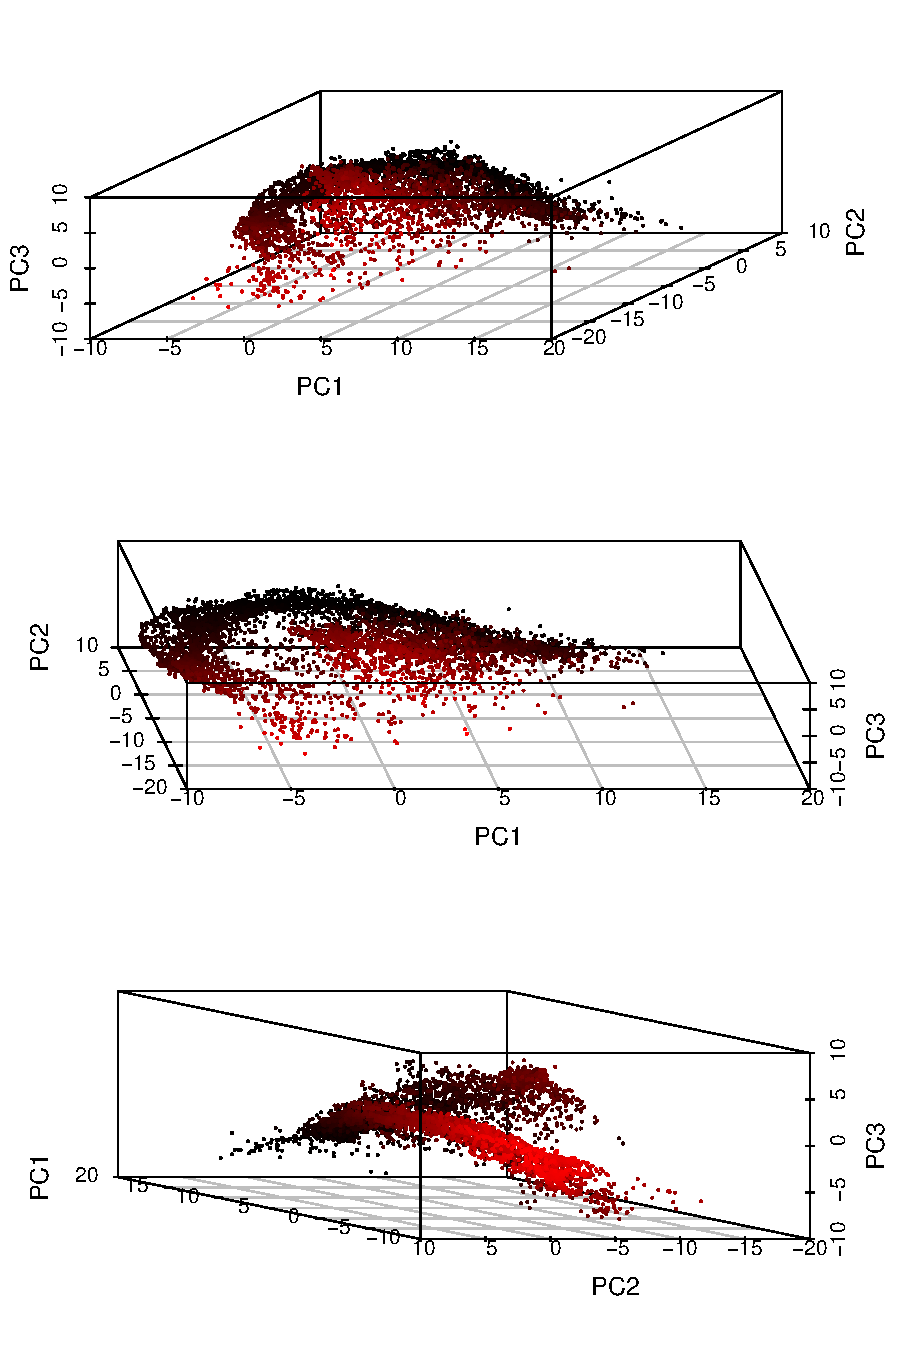
\includegraphics{niche-space-pca-3d}

These plots show that there are a few different clusters entangled with each other. At this stage I think some kind of clustering or nonlinear component decomposition is warranted. For now, I'm going to see if I can go learn something about kernel pca and related techniques.


\end{document}
